%%
%% This is file `tikzposter-template.tex',
%% generated with the docstrip utility.
%%
%% The original source files were:
%%
%% tikzposter.dtx  (with options: `tikzposter-template.tex')
%%
%% This is a generated file.
%%
%% Copyright (C) 2014 by Pascal Richter, Elena Botoeva, Richard Barnard, and Dirk Surmann
%%
%% This file may be distributed and/or modified under the
%% conditions of the LaTeX Project Public License, either
%% version 2.0 of this license or (at your option) any later
%% version. The latest version of this license is in:
%%
%% http://www.latex-project.org/lppl.txt
%%
%% and version 2.0 or later is part of all distributions of
%% LaTeX version 2013/12/01 or later.
%%


\documentclass{tikzposter} %Options for format can be included here

\usepackage{todonotes}

\usepackage[tikz]{bclogo}
\usepackage{lipsum}
\usepackage{amsmath}
\usepackage{fontawesome}
\usepackage{booktabs}
\usepackage{longtable}
\usepackage[absolute]{textpos}
\usepackage[it]{subfigure}
\usepackage{graphicx}
\usepackage{cmbright}
%\usepackage[default]{cantarell}
%\usepackage{avant}
%\usepackage[math]{iwona}
\usepackage[math]{kurier}
\usepackage[T1]{fontenc}
\usepackage{tikz}
%% add your packages here
\usepackage{hyperref}
% for random text
\usepackage{lipsum}
\usepackage[english]{babel}
\usepackage[pangram]{blindtext}
%\usepackage{smartdiagram}
\usepackage{forest}
%\usetikzlibrary{arrows.meta, shapes.geometric, calc, shadows}
\usepackage{pgfplots}
\usepackage[utf8]{inputenc}
\usepackage{dtk-logos}
\usepackage{tikz}
\usepackage{multirow}
\usepackage{multicol}
%\usepackage{outlines}
\usepackage{float}
\usepackage{subfigure}
\usepackage{tabularx}

\usetikzlibrary{arrows,chains,mindmap,shadows,automata,patterns,petri,shapes.geometric,shapes.misc, spy, trees,decorations.markings,positioning}
%\usepackage[hidelinks,pdfencoding=auto]{hyperref}
% Information boxes
\newcommand*{\info}[4][4]{%
	\node [ annotation, #3, text width = 7cm,
	inner sep = 0.3em ] at (#2) {%
		\list{$\bullet$}{\topsep=-3pt\itemsep=0pt\parsep=1pt
			\parskip=1pt\labelwidth=0pt\leftmargin=1pt
			\itemindent=1pt\labelsep=1pt}%
		#4
		\endlist
	};
}

\usepackage{enumitem}

% aiming high
\usepackage{smartdiagram}
\usetikzlibrary{shapes.symbols}

\tikzset{description title/.append style={
		signal,
		signal to=north,
		signal from=south,
		yshift=0.5cm,
	}
}

\definecolor{mynodecolor}{RGB}{198,191,234}

%\pgfdeclarelayer{backgroundlayer}
%\pgfdeclarelayer{notelayer}

%forest
\usepackage{forest}
\usetikzlibrary{arrows.meta, shapes.geometric, calc, shadows}
\colorlet{mygreen}{green!75!black}
\colorlet{col1in}{red!30}
\colorlet{col1out}{red!40}
\colorlet{col2in}{mygreen!40}
\colorlet{col2out}{mygreen!50}
\colorlet{col3in}{blue!30}
\colorlet{col3out}{blue!40}
\colorlet{col4in}{mygreen!20}
\colorlet{col4out}{mygreen!30}
\colorlet{col5in}{blue!10}
\colorlet{col5out}{blue!20}
\colorlet{col6in}{blue!20}
\colorlet{col6out}{blue!30}
\colorlet{col7out}{orange}
\colorlet{col7in}{orange!50}
\colorlet{col8out}{orange!40}
\colorlet{col8in}{orange!20}
\colorlet{linecol}{blue!60}



% Title, Author, Institute
\title{Team for Universal Learning and Intelligent Processing}
\institute{TULIP Academy}
%\author{Gang Li}
%\institute{School of Information Technology \\
%Deakin University, Australia
%}
%\titlegraphic{logos/tulip-logo.eps}

%Choose Layout
\usetheme{Wave}

%\definebackgroundstyle{samplebackgroundstyle}{
%\draw[inner sep=0pt, line width=0pt, color=red, fill=backgroundcolor!30!black]
%(bottomleft) rectangle (topright);
%}\pgfdeclarelayer{background}
\pgfdeclarelayer{background}
\pgfdeclarelayer{foreground}
\pgfsetlayers{backgroundlayer,background,main,foreground,notelayer}
%

\colorlet{backgroundcolor}{blue!10}

\begin{document}
	
	\colorlet{blocktitlebgcolor}{blue!23}
	
	% Title block with title, author, logo, etc.
	\maketitle
	
	\begin{columns}
		% FIRST column
		\column{0.5}% Width set relative to text width
		
		%%%%%%%%%% -------------------------------------------------------------------- %%%%%%%%%%
		%\block{Main Objectives}{
		%  	      	\begin{enumerate}
		%  	      	\item Formalise research problem by extending \emph{outlying aspects mining}
		%  	      	\item Proposed \emph{GOAM} algorithm is to solve research problem
		%  	      	\item Utilise pruning strategies to reduce time complexity
		%  	      	\end{enumerate}
		%%  	      \end{minipage}
		%}
		%%%%%%%%%% -------------------------------------------------------------------- %%%%%%%%%%
		
		
		%%%%%%%%%% -------------------------------------------------------------------- %%%%%%%%%%
		\block{TULIP Academy}{
			\selectcolormodel{rgb}
			\pgfkeys{/forest,
				rect/.append style   = { rounded corners = 2pt,
					inner color = blue!30, outer color = blue!30},
				ellip/.append style  = { inner color = blue!30,
					outer color = blue!30},
				orect/.append style  = { font = \sffamily\bfseries\small,
					text width = 325pt, text centered,
					minimum height = 10pt, outer color = blue!30,
					inner color=blue!30},
				oellip/.append style = { inner color = blue!30, outer color = blue!30,
					font = \sffamily\bfseries\small, text centered}}
		\begin{minipage}[l]{0.35\linewidth}
			\begin{center}
				\begin{description}[font=\small]
					%\centering
					\item[Official Websites] \hfill
					\begin{itemize}
						\footnotesize \item \textcolor{orange}{\faHome:} http://www.tulip.org.au
						\item \textcolor{orange}{\faGithub:} https://github.com/tulip-lab
					\end{itemize}						
					\item[Social Media] \hfill
					\begin{itemize}
						\footnotesize \item \textcolor{orange}{\faTwitter:} tulipacademy
						\item \textcolor{orange}{\faWeibo:} tulipacademy
						\item \textcolor{orange}{\faRedditAlien:} https://www.reddit.com/r/tulipacademy
					\end{itemize}
					
					
					\item[Internal Services] \hfill
					\begin{itemize}
						\footnotesize \item \textcolor{orange}{\faBitbucket:} https://bitbucket.org
						\item \textcolor{orange}{\faCalendar:} https://goo.gl/cWCWwC
						\item \textcolor{orange}{\faCalendarCheckO:} https://goo.gl/aC9VWW (iCal)
					\end{itemize}
					
				\end{description}
			\end{center}				
		\end{minipage}
		\hfill
		\begin{minipage}[l]{0.65\linewidth}
			\scalebox{0.9}[1]	{
				\begin{forest}
					for tree={
						font=\sffamily\bfseries\small,
						line width=1pt,
						%      draw=linecol,
						ellip,
						align=center,
						child anchor=north,
						parent anchor=south,
						drop shadow,
						l sep+=12.5pt,
						edge path={
							\noexpand\path[color=gray, rounded corners=5pt,
							>={Stealth[length=11pt]}, line width=1pt, ->, \forestoption{edge}]
							(!u.parent anchor) -- +(0,-5pt) -|
							(.child anchor)\forestoption{edge label};
						},
						where level={3}{tier=tier3}{},
						where level={0}{l sep-=5pt}{},
						where level={1}{}{},
					}
					[TULIP Academy %inner color=col1in, outer color=col1out
					[Visitor]
					[Flipper
					[Trainee
					[FLIP (00)]
					[\dots]
					[FLIP (05)] 	
					]								
					]
					[TULIP Lab
					[Australia]
					[China]
					[India]]
					[Alumni] %inner color =col7in, outer color = col7out]
					[Web Team] %, inner color=col2in, outer color=col2out]
					]
				\end{forest}							
			}		
		\end{minipage}							
		}
		%%%%%%%%%% -------------------------------------------------------------------- %%%%%%%%%%
		
		
		%%%%%%%%%% -------------------------------------------------------------------- %%%%%%%%%%
		\block{Research @ TULIP}{
			\begin{minipage}[l]{0.35\linewidth}
				\begin{center}
					\begin{description}[font=\small]			
						\item[Behavior Informatics] \hfill
						\begin{itemize}
							\footnotesize \item Identify anomaly in group behavior,
							such as \textit{astroturfing}, \textit{cyber-bullying} etc.
							\item Detect the periodical behavior from various check-in history
							\item Design suitable strategy to implement intended effects
						\end{itemize}
						\item[Data Privacy] \hfill
						\begin{itemize}
							\footnotesize \item Protect the individual private information
							which may be disclosed from data analytics, data release etc.
							\item Check the compliance of GDPR when accessing, releasing and transferring data
							across the countries
						\end{itemize}
						\item[Business Intelligence] \hfill
						\begin{itemize}
							\footnotesize \item Smart-farm data analytics
							\item Tourism and Hospitality management
							\item Recommendation System
						\end{itemize}
					\end{description}
				\end{center}				
			\end{minipage}
			\hfill
			\begin{minipage}[l]{0.6\linewidth}
				\scalebox{0.6}{
				\begin{tikzpicture}[ every annotation/.style = {draw,
				fill = white}]
					\path[mindmap,concept color=blue!30,font=\sffamily\bfseries,
					every node/.style={concept},root/.style    = {concept color=blue!30, font=\Large\bfseries,text width=13em},
					level 1 concept/.append style={font=\bfseries, sibling angle=110,text width=10em,level distance=9em,inner sep=0pt},
					level 2 concept/.append style={font=\sf,text width=8em, sibling angle=100, inner sep=0pt, level distance=7em},]
					node[root,scale=0.6, text=white] {Research Themes} [clockwise from=190]
					child[concept color=blue!30, text=black!90] {
						node[scale=0.6] {Behavior Informatics} [clockwise from=200]
						child { node[scale=0.6] (pbm){Periodic Behavior Mining}}
						child { node[scale=0.6] (bp) {Group Anomaly Detection}}
					}
					child[concept color=blue!30, text=black!90] {
						node[concept,scale=0.6] {Data Privacy}[clockwise from=120]
						child{node[concept,scale=0.6](dcc){Compliance Checking}}
						child{node[concept,scale=0.6](privacy){Information Abuse Prevention}}
					}
					child[concept color=blue!30, text=black!90] {
						node[concept,scale=0.6] {Business Intelligence}[clockwise from=60]
						child{node[concept,scale=0.6](rs){Recommender System} }
						child{node[concept,scale=0.6](thm){Tourism \& Hospitality Management}}
					}
					;

				\end{tikzpicture}
			}
			\end{minipage}
	
		}
		%%%%%%%%%% -------------------------------------------------------------------- %%%%%%%%%%
		
		%%%%%%%%%% -------------------------------------------------------------------- %%%%%%%%%%
		\block[titleleft]{Publications}
		{
%			\begin{multicols}{2}
					\begin{minipage}{\linewidth}
						%\selectcolormodel{rgb}
						\centering
						%\scalebox{1}
						{
							\begin{tikzpicture}
							\begin{axis}[x=2.3cm, y=1.05cm,
							xtick={2006,2008,2010,2012, 2014, 2016, 2018}, 
							ytick={0,2,4,6,8,10,12,14},   
							x tick label style={rotate=75,anchor=east,/pgf/number format/1000 sep=},
							legend pos=north west, xmajorgrids=true, ymajorgrids=true, grid style=dashed, ]
							\addplot[mark=*,draw=blue, ultra thick]
							coordinates {
								(2006,0)(2007,1)(2008,3)(2009,2)(2010,5)(2011,9)
								(2012,5)(2013,12)(2014,12)(2015,11)(2016,6)(2017,9)(2018,12)
							};
							\addlegendentry{\footnotesize{SCI/SSCI Journals}}
							
							\addplot[mark=square,draw=orange,ultra thick]
							coordinates {
								(2006,2)(2007,3)(2008,6)(2009,4)(2010,3)(2011,2)(2012,7)
								(2013,7)(2014,4)(2015,3)(2016,5)(2017,6)(2018,5)
							};
							\addlegendentry{\footnotesize{Referred Conferences}}
							\end{axis}
							\end{tikzpicture}		
						}		
					\end{minipage}
				
				\vspace{1cm}
				
				\scalebox{1}
				{
					\begin{minipage}{\linewidth}
						\setlength{\abovecaptionskip}{-25pt}
						\setlength{\belowcaptionskip}{12pt}
						%\caption{TULIP Lab Publications}
						%\fontsize{13pt}{14pt}\selectfont
						\centering
						\setlength{\tabcolsep}{0.8cm}{
						\begin{tabular}{c|c c c|c c c}
							\toprule
							\cmidrule{1-1}    \multirow{2}[4]{*}{Year} & \multicolumn{3}{c}{SCI/SSCI Journals} &\multicolumn{3}{c}{Referred Conferences} \\
							\cmidrule{2-7}          & Q1 (71\%) & Q2 (18\%) & Q3 (11\%) & A (16\%) & B (9\%) & C (75\%) \\
							\midrule
							2018  & 9     & 1     & 2     & 0     & 1     & 4 \\
							2017  & 6     & 2     & 1     & 0     & 0     & 6 \\
							2016  & 2     & 3     & 1     & 0     & 0     & 5 \\
							2015  & 6     & 4     & 1     & 0     & 1     & 2 \\
							2014  & 10    & 0     & 2     & 0     & 0     & 4 \\
							2013  & 11    & 1     & 0     & 3     & 2     & 2 \\
							2012  & 2     & 1     & 2     & 4     & 1     & 2 \\
							2011  & 7     & 1     & 1     & 0     & 0     & 2 \\
							2010  & 4     & 1     & 0     & 2     & 0     & 1 \\
							2009  & 1     & 1     & 0     & 0     & 0     & 4 \\
							2008  & 3     & 0     & 0     & 0     & 0     & 6 \\
							2007  & 1     & 0     & 0     & 0     & 0     & 3 \\
							2006  & 0     & 0     & 0     & 0     & 0     & 2 \\
							\bottomrule
						\end{tabular}}
					\end{minipage}
				}	
				
%			\end{multicols}
		}
		%%%%%%%%%% -------------------------------------------------------------------- %%%%%%%%%%
		
		\column{0.5}
		%%%%%%%%%% -------------------------------------------------------------------- %%%%%%%%%%
		\block{Training @ TULIP}{
			\begin{minipage}[l]{0.6\linewidth}
				\centering
				\scalebox{0.7}{
					\begin{tikzpicture}[ every annotation/.style = {draw,
						fill = white}]
						\path[mindmap,concept color=blue!30,font=\sffamily\bfseries,
						every node/.style={concept},
						root/.style    = {concept color=blue!30,
							font=\Large\bfseries,text width=9em},
						level 1 concept/.append style={font=\bfseries,
							sibling angle=100,text width=7.7em,level distance=8em,inner sep=0pt},
						level 2 concept/.append style={font=\sf,text width=5em,inner sep=0pt, level distance=6em},
						]
						node[root,scale=0.6, text=white] {Research Training} [clockwise from=187]
					child[concept color=blue!30,text=black!90] {
						node[scale=0.6] {Professional Skills} [clockwise from=290]
						child { node[scale=0.6] (goReview) {Time Management}}
						child { node[scale=0.6] (goRefrences ){References Management}}
						child { node[scale=0.6] {\LaTeX}}
						child { node[scale=0.6] (goVersionCon) {Version Control System}}
					}
					child[concept color=blue!30,text=black!90] {
						node[concept,scale=0.6] {FLIP}[clockwise from=160]
						child{node[concept,scale=0.6](hand-on){Hand-on Skills}}
						child{node[concept,scale=0.6](Professional){Professional Knowledge}}
						child{node[concept,scale=0.6](Theo){Theoretical knowledge}}
						child{node[concept,scale=0.6](Math){Mathmatics}}
					}
					child[concept color=blue!30,text=black!90] {
						node[concept,scale=0.6] {Research Skills}
						[clockwise from=60]
						child { node[concept,scale=0.6] (TeXampleBlog){Reading}}
						child { node[concept,scale=0.6] (Reviewteam){Reviewing}}
						child { node[concept,scale=0.6] (present){Writing}}
						child { node[concept,scale=0.6] (write){Presenting}}
					}
					;
%					\info{Theo.north east}{above,anchor=west, yshift=-1.8em, xshift=1.0em}{%
%						\item FLIP (00): Data Science
%						\item FLIP (01): Advanced Data Science
%						\item FLIP (02): Modern Data Science
%						\item FLIP (03): Deep Learning
%						\item FLIP (04): Learning Theory (I)
%						\item FLIP (05): Learning Theory (II)
%						\item FLIP (06): Reading Team
%						\item FLIP (07): Review Team
%						\item FLIP (X): $\infty$
%					}
					\end{tikzpicture}
				}
			\end{minipage}
			\hfill
			\hspace{-0.005\textwidth}
			\begin{minipage}[l]{0.35\linewidth}
				\vspace{-30pt}
				\begin{center}
					\begin{description}[font=\small]			
						\item[Flipper] \hfill
						\begin{itemize}
							\footnotesize 
							\item FLIP (00): Data Science
							\item FLIP (01): Advanced Data Science
						\end{itemize}
						\item[Trainee] \hfill
						\begin{itemize}
							\footnotesize 
							\item FLIP (02): Modern Data Science
							\item FLIP (03): Deep Learning
						\end{itemize}
						\item[$\infty$] \hfill
						\begin{itemize}
							\footnotesize 
							\item FLIP (04): Learning Theory (I)
							\item FLIP (05): Learning Theory (II)
							\item FLIP (06): Reading Team
							\item FLIP (07): Review Team
							\item FLIP (X): $\infty$
						\end{itemize}
					\end{description}
				\end{center}				
			\end{minipage}
		}
		%%%%%%%%%% -------------------------------------------------------------------- %%%%%%%%%%
		
		
		
		%%%%%%%%%% -------------------------------------------------------------------- %%%%%%%%%%
		
		% Second column - second block
		\block[titleleft]{Minimum Requirements}
		{
			\begin{minipage}[l]{0.45\linewidth}
				\vspace{-30pt}
				\begin{description}[font=\small]
					\item[Honors or Master Students] \hfill
					\begin{itemize}
						\footnotesize \item $1$ \textcolor{orange}{CCF C} (or above) conference publication
						\item $1$ \textcolor{orange}{$Q_1$ journal} paper
					\end{itemize}
					\begin{description}[font=\small]
						\item[Deakin PhD Scholarship]  \hfill
						\begin{itemize}
							\footnotesize \item $2$ \textcolor{orange}{$Q_1$ journal} papers as the first author
							\item \textit{IELTS} overall $6.5$ with no band below $6$
						\end{itemize}
					\end{description}
					\item[PhD Students] \hfill
					\begin{itemize}
						\footnotesize \item $1$ research proposal
						\item $2$ \textcolor{orange}{CCF B} (or above) conference papers
						\item $2$ \textasciitilde{} $3$ \textcolor{orange}{ACM/IEEE Transactions},
						with impact factors added up to $5$
					\end{itemize}
					\item[Post-doctoral Research Fellows] \hfill
					\begin{itemize}
						\footnotesize \item \textit{annually} $1$ \textcolor{orange}{CCF A} and $1$ \textcolor{orange}{CCF B} conference papers
						\item \textit{annually} $4$ \textcolor{orange}{$Q_1$ journal} papers,
						with at least $1$ \textcolor{orange}{ACM/IEEE Transactions} paper
					\end{itemize}
					
				\end{description}		
			\end{minipage}
			\hfill
			\hspace{0.005\textwidth}
			\begin{minipage}[l]{0.55\linewidth}
				\vspace{-20pt}
				\scalebox{0.7}[0.75]{
					\smartdiagramset{description title width=5cm,
						set color list={blue!45,blue!30,blue!15},
						description title text width=4.5cm,
						descriptive items y sep=6.5cm,
						description text width=20cm,
						module minimum height=5.2cm}
					
					\smartdiagram[descriptive diagram]{
						{\textbf{$\infty$}, \begin{enumerate}
								\item Proactively meet with supervisor twice per week
								\item Proactively present and criticize at \textit{TULIP Seminar}
								\item FLIP (04-05) and FLIP (06-07) completion
								\item Act as FLIP team leaders and update materials annually
						\end{enumerate}},
						{\textbf{Trainee}, \begin{enumerate}
								\item FLIP (02-03) with success on open Kaggle projects
								\item Feedback and suggestions on FLIP
								\item Present at \textit{TULIP Seminar}
						\end{enumerate}},
						{\textbf{Flipper},\begin{enumerate}
								\item \LaTeX + \faGithub \faBitbucket + Time management + PPR skill
								\item Keep FLIP materials confidential without distribution
								\item FLIP (00-01) with success on open Kaggle projects
								\item Attend \textit{TULIP Seminar} with preparation and questions
						\end{enumerate}},}
				}
			\end{minipage}

			
		}
		%%%%%%%%%% -------------------------------------------------------------------- %%%%%%%%%%		
		
		%%%%%%%%%% -------------------------------------------------------------------- %%%%%%%%%%		
		\block[titleleft]{Awards}
		{
			\begin{minipage}{\linewidth}
				\begin{multicols}{3}
				\centering
				\begin{minipage}{\linewidth}
					\centering
					%\includegraphics[width=0.9\textwidth]{figures//awards//TULIPAwards2018B.eps}
					
\includegraphics[width=0.9\textwidth]{figures//awards//TULIPAwards2014.eps}
				\end{minipage}
				
				\begin{minipage}{\linewidth}
					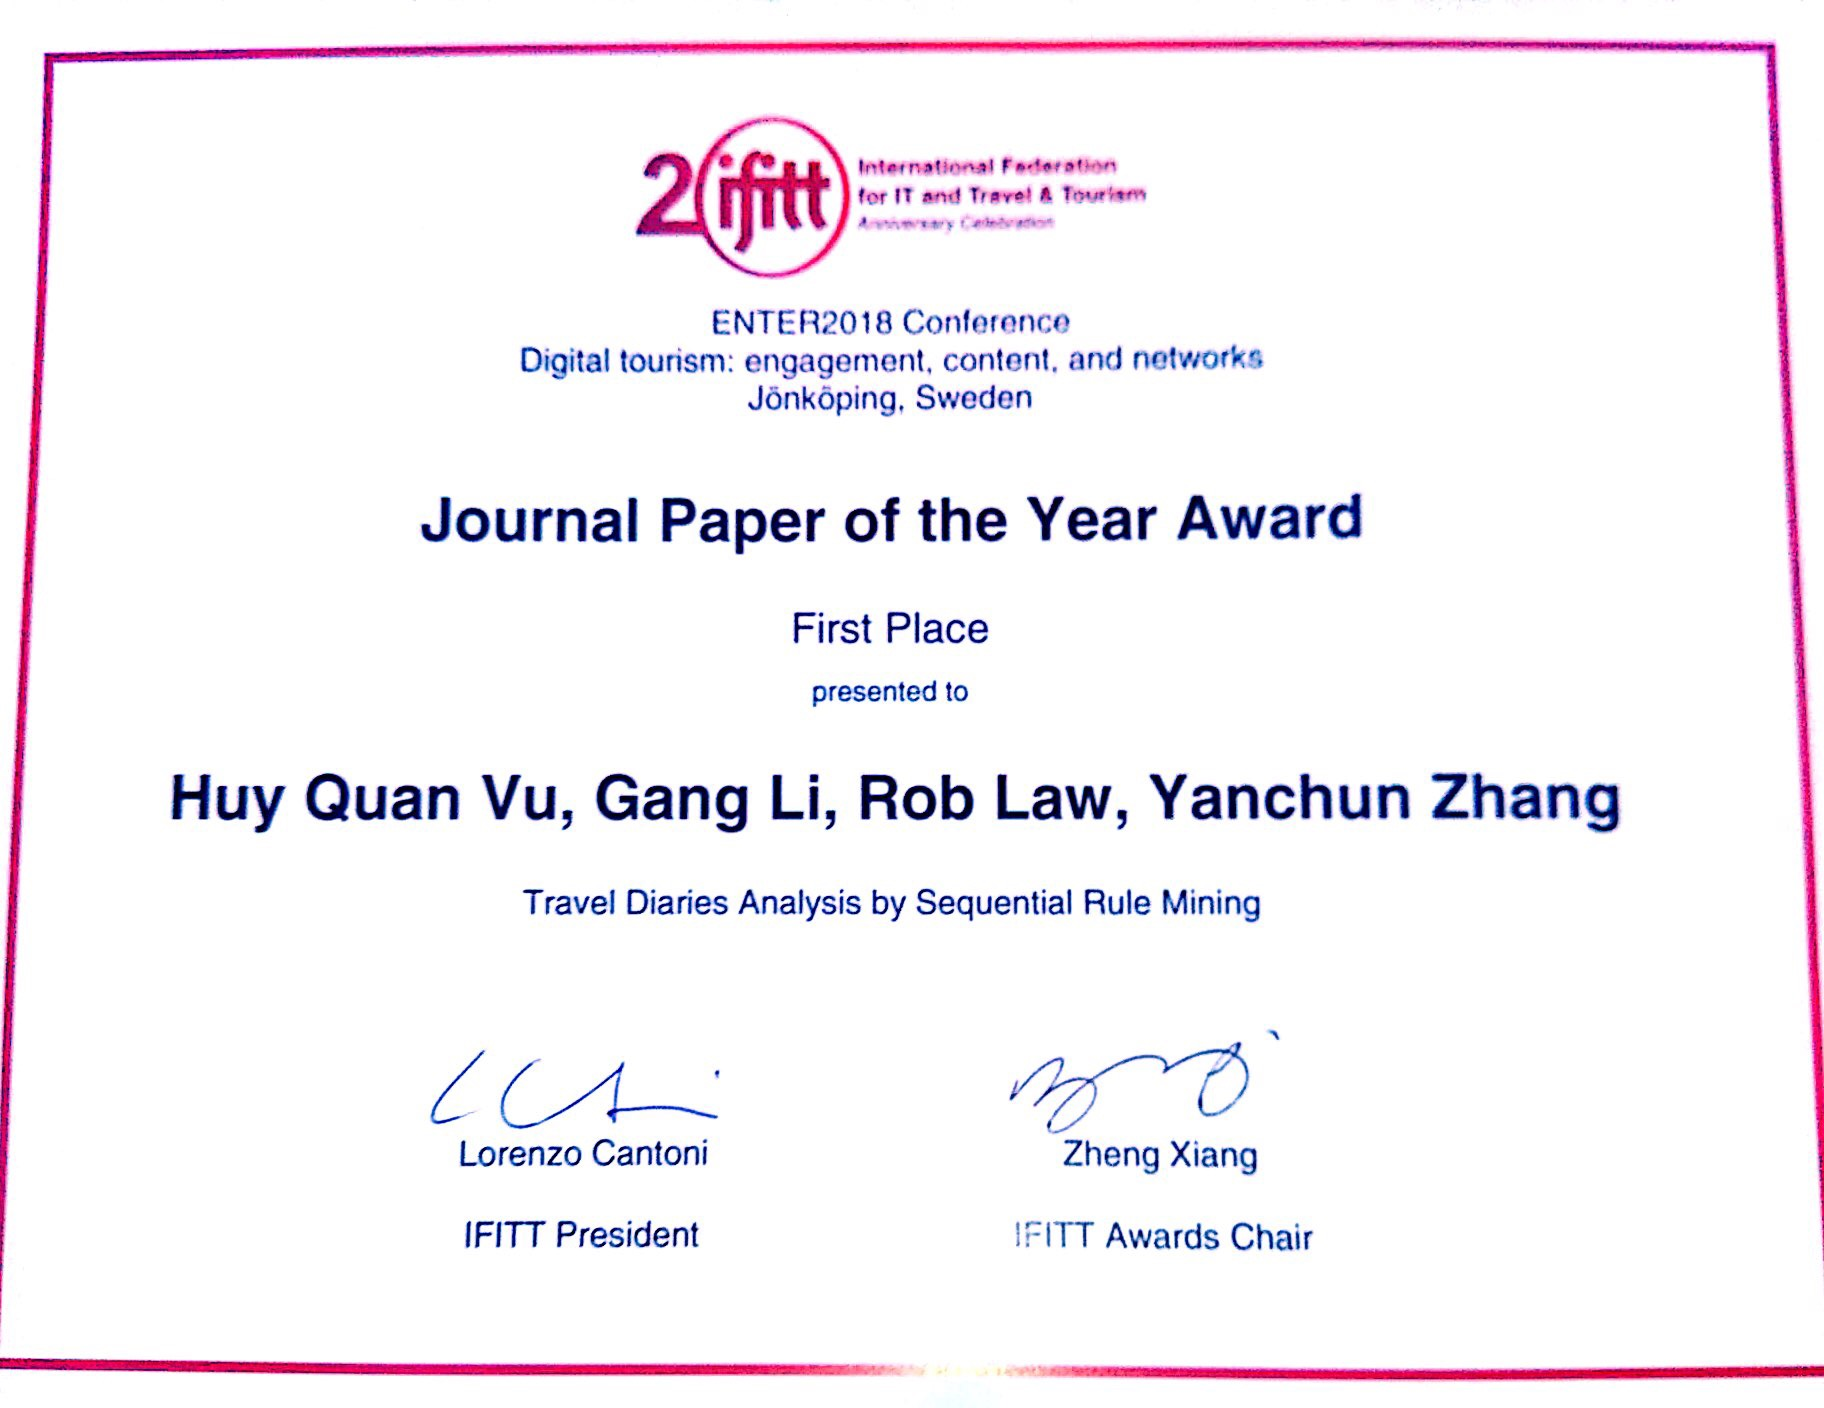
\includegraphics[width=0.85\textwidth]{figures//awards//TULIPAwards2018A.eps}
				\end{minipage}	
				
				\begin{minipage}{\linewidth}
					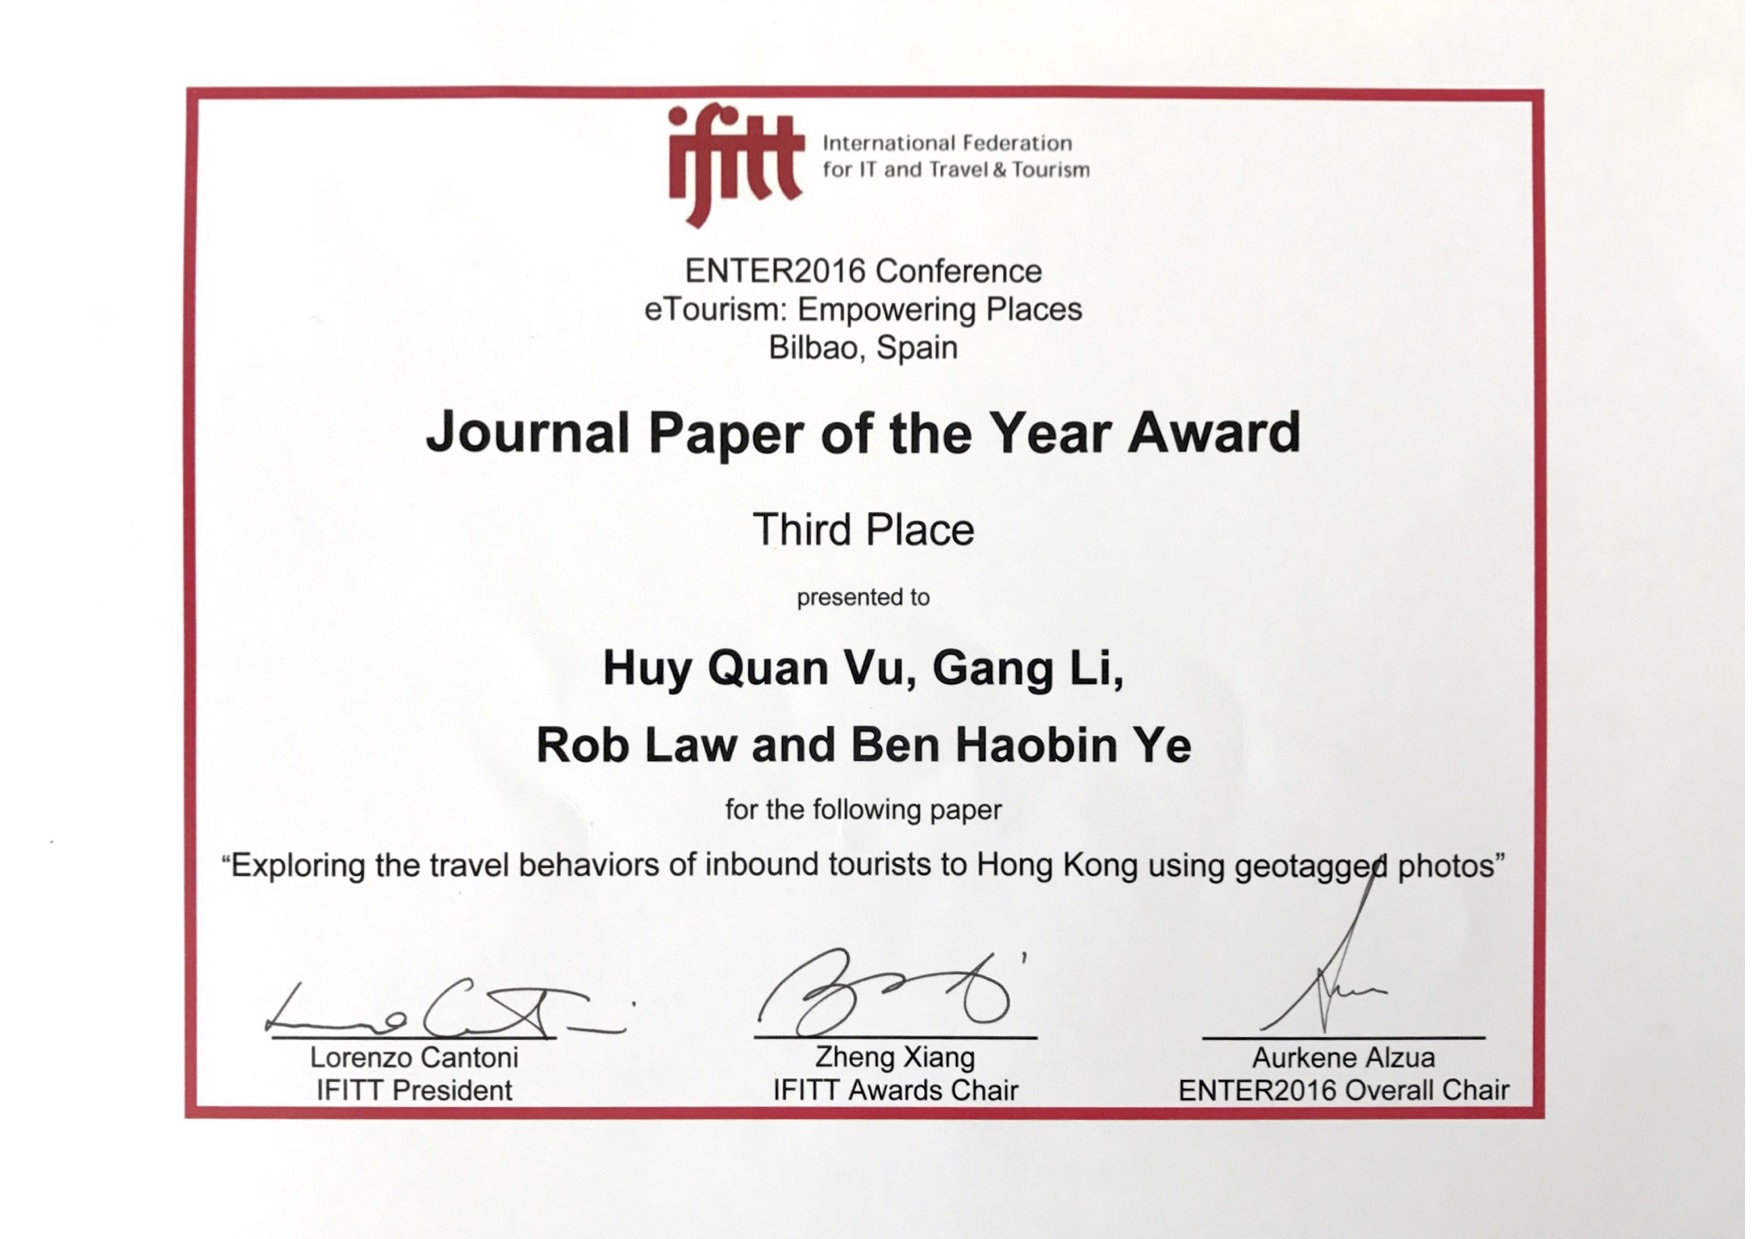
\includegraphics[width=\textwidth]{figures//awards//TULIPAwards2016A.eps}
				\end{minipage}				
				\end{multicols}
			\end{minipage}
			
			\vspace{0.6cm}
						
			\begin{minipage}{\linewidth}
				\begin{multicols}{3}
				\centering
				\begin{minipage}{\linewidth}
					\centering
					
\includegraphics[width=0.9\textwidth]{figures//awards//TULIPAwards2012.eps}
				\end{minipage}
				
				\begin{minipage}{\linewidth}
					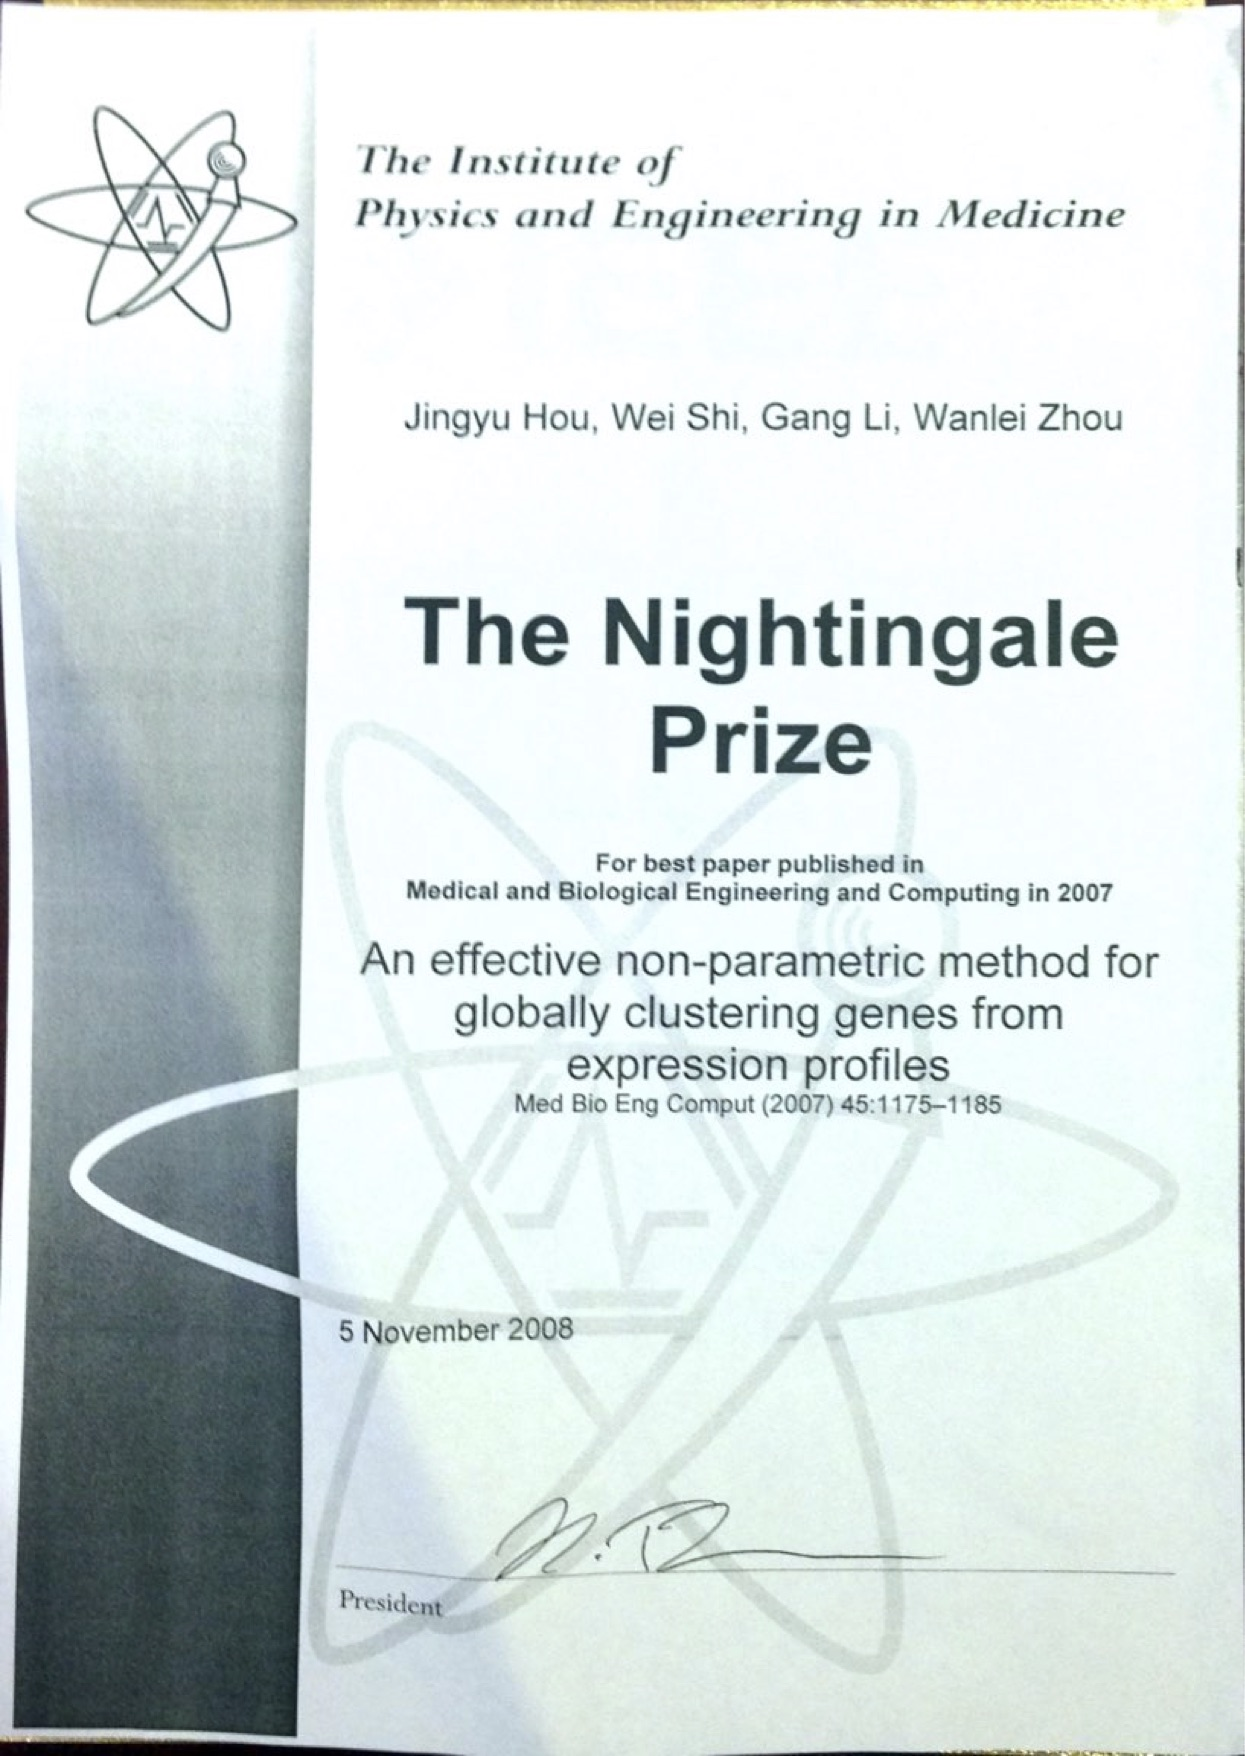
\includegraphics[width=0.9\textwidth]{figures//awards//TULIPAwards2007.eps}
				\end{minipage}				
				
				\begin{minipage}{\linewidth}
				\begin{figure}[H] 
					\begin{minipage}{\linewidth}
					\subfigure
					{ 
						
\includegraphics[width=0.84\textwidth]{figures//awards//TULIPAwards2016B.eps}
					}
					\end{minipage}
					\begin{minipage}{\linewidth}
					\subfigure
					{						
						\includegraphics[width=0.84\textwidth]{figures//awards//TULIPAwards2018B.eps}
					}
					\end{minipage}
				\end{figure}	
				\end{minipage}	
				\end{multicols}
			\end{minipage}
			
			\vspace{1.1cm}
			
			\scalebox{1}
			{
				\begin{minipage}{\linewidth}
					%\begin{table}[htbp]
					 \centering
					%  \caption{TULIP Lab Research Awards}
					\begin{tabular}{ r | l | r  r }
						\toprule
						\multicolumn{1}{ l |}{\textbf{Year}} & \textbf{Awards} & \textbf{Author} &  \\
						\midrule
						\textbf{2018} & KSEM 2018 \textit{Best Paper} Award & Shaoni Wang &  \\
						
						\textbf{2017} & IFITT \textit{Journal Paper of The Year} Award (1st Prize) & Huy Quan Vu &  \\
						
						\textbf{2016} & IEEE TrustCom 2016 \textit{Best Student Paper} Award & Na Pang &  \\
						
						\textbf{2015} & IFITT \textit{Journal Paper of The Year} Award (3rd Prize) & Huy Quan Vu &  \\
						
						\textbf{2014} & PAKDD 2014 \textit{Best Student Paper} Award & Tianqing Zhu &  \\
						
						\textbf{2012} & ACM ASONAM 2012  \textit{Best Paper} Award & Yongli Ren &  \\
						
						\textbf{2007} & Springer 2007 \textit{Nightingale Prize} & Jingyu Hou &  \\
						\bottomrule
					\end{tabular}
					%\end{table}
				\end{minipage}
			}		
		}
		%%%%%%%%%% -------------------------------------------------------------------- %%%%%%%%%%
		
		
		% Bottomblock
		%%%%%%%%%% -------------------------------------------------------------------- %%%%%%%%%%
		%\colorlet{notebgcolor}{blue!20}
		%\colorlet{notefrcolor}{blue!20}
		%\note[targetoffsetx=8cm, targetoffsety=-4cm, angle=30, rotate=15,
		%radius=2cm, width=.26\textwidth]{
		%Acknowledgement
		%\begin{itemize}
		%    \item
		%    International Cooperation Project (Y7Z0511101)
		%    of IIE,
		%    Chinese Academy of Sciences
		% \end{itemize}
		%}
		
		%\note[targetoffsetx=8cm, targetoffsety=-10cm,rotate=0,angle=180,radius=8cm,width=.46\textwidth,innersep=.1cm]{
		%Acknowledgement
		%}
		
		%\block[titlewidthscale=0.9, bodywidthscale=0.9]
		%{Acknowledgement}{
		%}
		%%%%%%%%%% -------------------------------------------------------------------- %%%%%%%%%%
		
	\end{columns}
	
	
	%%%%%%%%%% -------------------------------------------------------------------- %%%%%%%%%%
	%[titleleft, titleoffsetx=2em, titleoffsety=1em, bodyoffsetx=2em,%
	%roundedcorners=10, linewidth=0mm, titlewidthscale=0.7,%
	%bodywidthscale=0.9, titlecenter]
	
	%\colorlet{noteframecolor}{blue!20}
	\colorlet{notebgcolor}{blue!20}
	\colorlet{notefrcolor}{blue!20}
	\note[targetoffsetx=-13cm, targetoffsety=-24cm,rotate=0,
	angle=180,radius=8cm,width=.96\textwidth,innersep=.4cm]
	{
		\begin{minipage}{0.3\linewidth}
			\centering
			
\includegraphics[width=24cm]{logos/tulip-wordmark.eps}
		\end{minipage}
		\begin{minipage}{0.7\linewidth}
			{ \centering
%				\large{\textcolor{blue!80}{Welcome to \emph{Team for Universal Learning and
%							Intelligent Processing}!}}
			}
		\end{minipage}
	}
	%%%%%%%%%% -------------------------------------------------------------------- %%%%%%%%%%
	
\end{document}

\endinput
%%
%% End of file `tikzposter-template.tex'.
